% !TEX root = ../Grunddatei.tex
\section{Vorbereitung}

\subsection{Aktive und passive Zweipole}

Für einen aktiven Zweipol wurden nacheinander die Spannungen $U_1$, $U_2$ und der dazugehörige Strom $I_1$ bzw. $I_2$ gemessen.
Über das Ohm'sche Gesetz
\begin{equation*}
    \label{eq:ohmschesGesetz}
    U=R\cdot I
\end{equation*} kann der Widerstand $R$ berechnet werden. Die Ergebnisse sind in Tabelle \ref{tab:aktiveZweipole} zu sehen.
\begin{center}
    \begin{table}[ht]
        \begin{tabularx}{\linewidth}{|*{4}{X|}}
            \hline
            No. & $U$/V & $I$/A & R/${\Omega}$ \\
            \hline
            1   & 6,5   & 0,5   & 13           \\
            2   & 3,5   & 1,5   & 2,3          \\
            \hline
        \end{tabularx}
        \caption{Messwerte für aktive Zweipole}
        \label{tab:aktiveZweipole}
    \end{table}
\end{center}
Des Weiteren wurden die Leerlaufspannung $U_q$, der Kurzschlussstrom $I_k$ und der Innenwiderstand $R_i$ gemessen bzw. über die Beziehung
\begin{equation*}
    \label{eq:innenwiderstand}
    R_i=\frac{U_q}{I_k}
\end{equation*} berechnet.\\
Es ergeben sich die Kenngrößen $U_l=8\,$V,$I_k=2,67\,$A und $R_i=3\,\Omega$.

\subsection{Abgegebene Leistung des aktiven Zweipole}
Die abgegebene Leistung $P_a$ des aktiven Zweipols wird über die Formel
\begin{equation}
    \label{eq:abgegebeneLeistungAllgemein}
    P_a=U\cdot I
\end{equation}
bzw.
\begin{equation}
    \label{eq:abgegebeneLeistung}
    P_a=U_q^{2}\cdot{\frac{R_a}{(R_i+R_a)^2}}
\end{equation}
berechnet.\\
Im Diagramm \ref{fig:abgegebeneLeistung} ist die abgegebene Leistung $P_a$ in Abhängigkeit des Widerstands $R_a$ = (0\dots15) $\Omega$ nach \eqref{eq:abgegebeneLeistung} dargestellt.

\begin{figure}
    \centering
    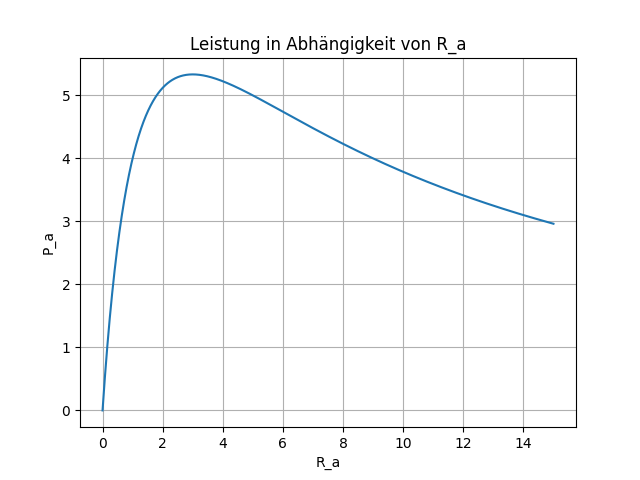
\includegraphics[width=0.8\linewidth]{Bilder/abgegebeneLeistung.png}
    \caption{Abgegebene Leistung $P_a$ in Abhängigkeit des Widerstands $R_a$}
    \label{fig:abgegebeneLeistung}
\end{figure}

\subsection{Anwendung des HELMHOLTZschen Überlagerungssatzes}\label{sec:helmholtz}

Zu bestimmen ist der Strom $I_{AB}$ in der Schaltung \ref{fig:helmholtzSchaltung} mit Hilfe des HELMHOLTZschen Überlagerungssatzes.

\begin{figure}[ht]
    \centering
    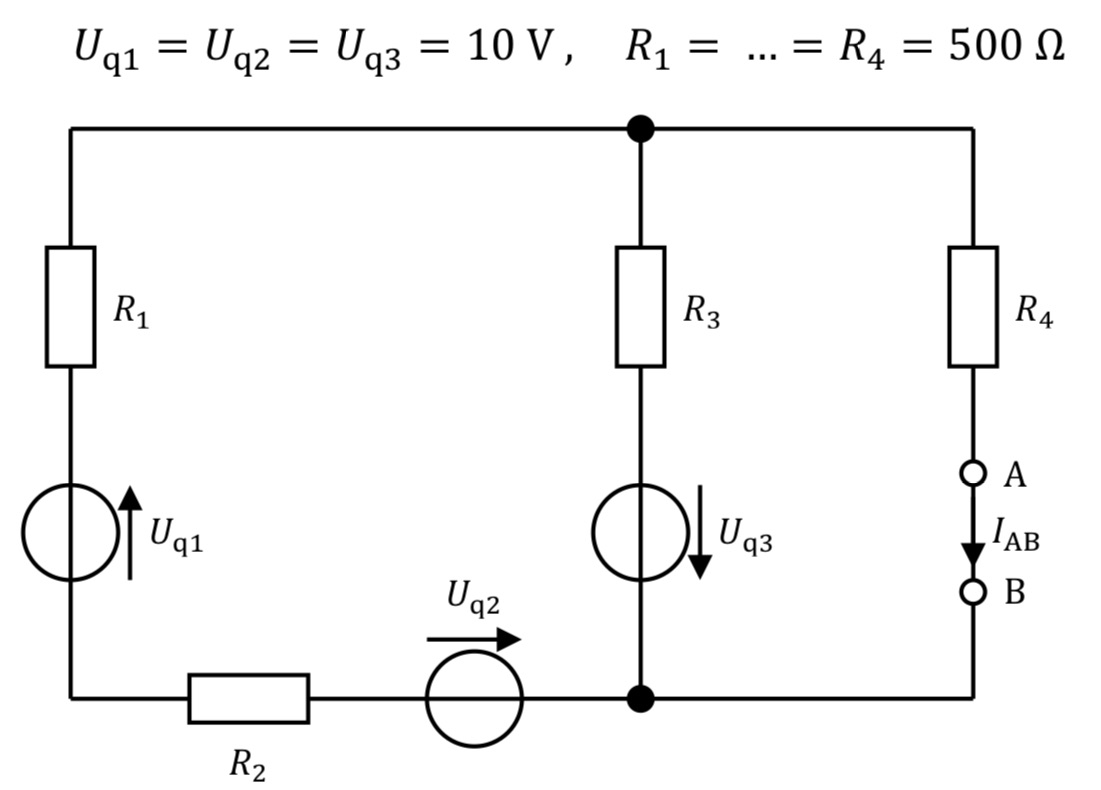
\includegraphics[width=0.5\linewidth]{Bilder/Helmholtz.png}
    \caption{Schaltung zur Anwendung des Überlagerungssatzes\cite{Anleitung}}
    \label{fig:helmholtzSchaltung}
\end{figure}

Dafür wird nacheinander eine Spannungsquelle ausgewählt und die anderen Spannungsquellen durch Kurzschlüsse ersetzt.\\
Für die Spannungsquelle $U_1$ mit $U_{q1}=10\,V$ ergibt sich zunächst der Gesamtwiderstand $R_{ges1}$ über
\begin{equation}
    \label{eq:gesamtwiderstand1}
    R_{ges1}=R_1+R_2+(R_3\parallel R_4)=1250\,\Omega\, .
\end{equation}
Somit ergibt sich über das Ohm'sche Gesetz der Strom $I_{AB1}$ zu
\begin{equation*}
    I_{1}=\frac{U_{q1}}{R_{ges1}}=8\,mA\, .
\end{equation*}
Wegen der Stromteilerregel gilt für die Beziehung zwischen $I_{AB1}$ und $I_{1}$
\begin{equation*}
    \frac{I_{AB1}}{I_{AB1}}=\frac{R_3}{R_3+R_4}
\end{equation*}
bzw.
\begin{equation}
    \label{eq:stromab1}
    I_{AB1}=\frac{R_3}{R_3+R_4}\cdot{I_{1}}=4\,mA\, .
\end{equation}

Für die Spannungsquelle $U_2$ mit $U_{q2}=10\,V$ ergibt sich zunächst mit $R_{ges2} = 1250\,\Omega$ der gleiche Gesamtwiderstand wie in \eqref{eq:gesamtwiderstand1}. Analog ergibt sich der Strom $I_{AB2}$ zu
\begin{equation}
    \label{eq:stromab2}
    I_{AB2}=\frac{R_4}{R_3+R_4}\cdot{I_{2}}=4\,mA\, .
\end{equation}

Für $U_3$ mit $U_{q3}=10\,V$ ergibt sich zunächst der Gesamtwiderstand $R_{ges3}$ über
\begin{equation*}
    R_{ges3}=R_3+(R_1+R_2)\parallel R_4=833\,\Omega\, .
\end{equation*}
Über die Stromteilerregel ergibt sich der Strom $I_{AB3}$ zu
\begin{equation}
    \label{eq:stromab3}
    I_{AB3}=\frac{R_1 + R_2}{R_1+R_2+R_4}\cdot{I_{3}}=12\,mA\, .
\end{equation}

Mit den Ergebnissen für $I_{AB1}$, $I_{AB2}$ und $I_{AB3}$ nach \eqref{eq:stromab1}, \eqref{eq:stromab2} und \eqref{eq:stromab3}  ergibt sich der Gesamtstrom $I_{AB}$ zu
\begin{equation*}
    I_{AB}=I_{AB2}+I_{AB3}-I_{AB1}=8\,mA\, .
\end{equation*}
Der Strom $I_{AB1}$ muss hierbei negativ betrachtet werden, da er in die entgegengesetzte Richtung fließt.



